%%%%%%%%%%%%%%%%%%%%%%%%%%%%%%%%%%%%%%%%%
% Beamer Presentation
% LaTeX Template
% Version 1.0 (10/11/12)
%
% This template has been downloaded from:
% http://www.LaTeXTemplates.com
%
% License:
% CC BY-NC-SA 3.0 (http://creativecommons.org/licenses/by-nc-sa/3.0/)
%
%%%%%%%%%%%%%%%%%%%%%%%%%%%%%%%%%%%%%%%%%

%----------------------------------------------------------------------------------------
%	PACKAGES AND THEMES
%----------------------------------------------------------------------------------------

\documentclass{beamer}

\mode<presentation> {

% The Beamer class comes with a number of default slide themes
% which change the colors and layouts of slides. Below this is a list
% of all the themes, uncomment each in turn to see what they look like.

%\usetheme{default}
%\usetheme{AnnArbor}
%\usetheme{Antibes}
%\usetheme{Bergen}
%\usetheme{Berkeley}
%\usetheme{Berlin}
%\usetheme{Boadilla}
%\usetheme{CambridgeUS}
%\usetheme{Copenhagen}
%\usetheme{Darmstadt}
%\usetheme{Dresden}
%\usetheme{Frankfurt}
%\usetheme{Goettingen}
%\usetheme{Hannover}
%\usetheme{Ilmenau}
%\usetheme{JuanLesPins}
%\usetheme{Luebeck}
\usetheme{Madrid}
%\usetheme{Malmoe}
%\usetheme{Marburg}
%\usetheme{Montpellier}
%\usetheme{PaloAlto}
%\usetheme{Pittsburgh}
%\usetheme{Rochester}
%\usetheme{Singapore}
%\usetheme{Szeged}
%\usetheme{Warsaw}

% As well as themes, the Beamer class has a number of color themes
% for any slide theme. Uncomment each of these in turn to see how it
% changes the colors of your current slide theme.

%\usecolortheme{albatross}
%\usecolortheme{beaver}
%\usecolortheme{beetle}
%\usecolortheme{crane}
%\usecolortheme{dolphin}
%\usecolortheme{dove}
%\usecolortheme{fly}
%\usecolortheme{lily}
%\usecolortheme{orchid}
%\usecolortheme{rose}
%\usecolortheme{seagull}
%\usecolortheme{seahorse}
%\usecolortheme{whale}
%\usecolortheme{wolverine}

%\setbeamertemplate{footline} % To remove the footer line in all slides uncomment this line
%\setbeamertemplate{footline}[page number] % To replace the footer line in all slides with a simple slide count uncomment this line

%\setbeamertemplate{navigation symbols}{} % To remove the navigation symbols from the bottom of all slides uncomment this line
}

\usepackage{graphicx} % Allows including images
\usepackage[absolute, overlay]{textpos}
\usepackage{booktabs} % Allows the use of \toprule, \midrule and \bottomrule in tables
\usepackage{tikz}
\usetikzlibrary{positioning,calc,backgrounds,shapes}

\usepackage[labelformat=empty]{caption}
\captionsetup{compatibility=false}

\tikzset{My Arrow Style/.style={single arrow, fill=red!30, anchor=base, align=center,text width=4cm}}
\newcommand{\arrowthis}[2][]{\tikz[baseline] \node [My Arrow Style,#1] {#2};}


\tikzset{My Speech Style/.style={ellipse callout, fill=red!50, anchor=base, align=center,text width=2.8cm}}
\newcommand{\speechthis}[2][]{
    \tikz[baseline]{\node[My Speech Style, #1]{#2};}
}%

\newcommand{\source}[1]{\begin{textblock*}{4cm}(8.7cm,8.2cm)
        \begin{beamercolorbox}[ht=0.5cm,right]{framesource}
        \usebeamerfont{framesource}\usebeamercolor[fg]{framesource} Source: {#1}
        \end{beamercolorbox}
    \end{textblock*}
}
%----------------------------------------------------------------------------------------
%	TITLE PAGE
%----------------------------------------------------------------------------------------

\title[University of Bucharest]{HTSeq - a Python framework to work with high-throughput sequencing data}
% The short title appears at the bottom of every slide, the full title is only on the title page
\author[Drago\c{s} Alin Rotaru]{Drago\c{s} Alin Rotaru} % Your name
\institute[UniBuc] % Your institution as it will appear on the bottom of every slide, may be shorthand to save space
{
University of Bucharest\\ % Your institution for the title page
% \medskip
}
\date{24 April, 2015} % Date, can be changed to a custom date

\begin{document}

\begin{frame}
\titlepage % Print the title page as the first slide
\end{frame}



\AtBeginSection[]
{
  \begin{frame}<beamer>
    \frametitle{Overview for section \thesection}
    \tableofcontents[currentsection]
  \end{frame}
}

%----------------------------------------------------------------------------------------
%	PRESENTATION SLIDES
%----------------------------------------------------------------------------------------

%------------------------------------------------
\section{Introduction} % Sections can be created in order to organize your presentation into discrete blocks, all sections and subsections are automatically printed in the table of contents as an overview of the talk
%------------------------------------------------

\begin{frame}
    \frametitle{Motivation}

    \begin{itemize}
        \item Low cost DNA sequencing
        \pause
        \item Technologies that can take a snapshot of RNA at a moment (RNA-Seq)
        \pause
        \item Size of human genome is about 3,234.83 Mb (Mega-basepairs) 
        \pause
        \item Dealing with HTS(High Throughput Sequencing) data is inevitably
    %\item Motivation; importance of DNA sequencing, RNA sequencing
    %insert some image with NGS
    \end{itemize}
\end{frame}

\section{Trying to solve HTSeq-data problems}

\begin{frame}
    \frametitle{Current problems} 
    \begin{itemize}
        \item Most tools are built only for specific purposes
        \pause
        \item Part of them: not open-source
        \pause
        \item Part of the others: not suitable for high performance tasks
    \end{itemize}
\end{frame}


\begin{frame}
    \frametitle{What is HTSeq?}
    \only<1-1> {
        \begin{itemize}
            \item Framework for Python
            \item Written in Cython
            \item Great and easy for writing customizable scripts
            \item High level scripts
            \item Well documented
        \end{itemize}
    }
    \only<2-> {
        \begin{textblock*}{10cm}(1cm, 1cm)
            \begin{figure}
                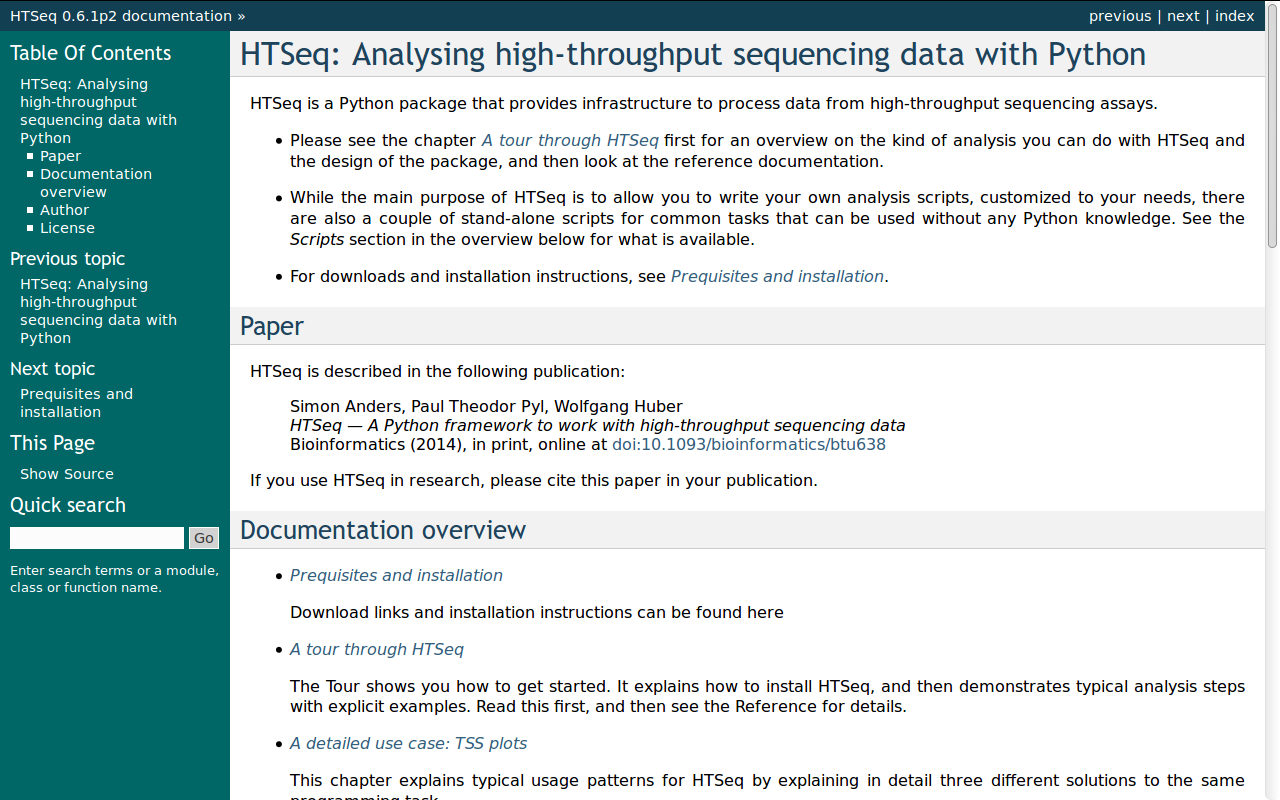
\includegraphics[width=10cm,height=10cm,keepaspectratio]{img/website.png}
                \caption{HTSeq - Documentation Website}
            \end{figure}
        \end{textblock*} 
    }
\end{frame}

\section{Prerequisites}

\begin{frame} 
    \frametitle{Back to biology... - Phred Quality Scores}
    \begin{textblock*}{10cm}(1cm, 1cm)
            \begin{figure}
                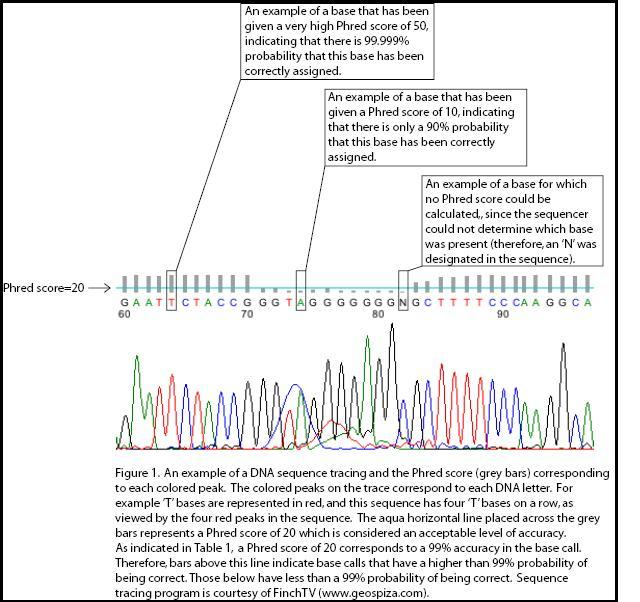
\includegraphics[width=10cm,height=7cm,keepaspectratio]{img/PhredFigure1.jpg}
                \caption{Phred Quality Scores - Source: Wiki}
            \end{figure}
    \end{textblock*}      
\end{frame}

\begin{frame}
    \frametitle{File formats?}
    \only<1-1> {
        \begin{itemize}
            \item FASTA files - representing nucleotide (A-C-G-T) or peptide (aminoacid) sequences 
            \item FASTQ files - usually nucleotide sequences, this time with their scores
        \end{itemize}
    }
\end{frame}


\begin{frame}[fragile]
\frametitle{File formats?}
\begin{verbatim}
@HWI-EAS209_0006_FC706VJ:5:58:5894:21141#ATCACG/1
TTAATTGGTAAATAAATCTCCTAATAGCTTAGATNTTACCTTNNNNNNNNNNTAGTTTCTTGAGATTTGTTGGGGGAGACATTTTTGTGATTGCCTTGAT
+HWI-EAS209_0006_FC706VJ:5:58:5894:21141#ATCACG/1
efcfffffcfeefffcffffffddf`feed]`]_Ba_^__[YBBBBBBBBBBRTT\]][]dddd`ddd^dddadd^BBBBBBBBBBBBBBBBBBBBBBBB
\end{verbatim}
\end{frame}

\begin{frame}
    \frametitle{More file formats}
    \begin{itemize}
        \item SAM - Sequence Alignments Map
        \pause
        \item SAM can be derived from FASTQ files by DNA aligning reads with some reference genome
    \end{itemize}

\end{frame}

\begin{frame}
\frametitle{More file formats}
    \begin{itemize}
        \item BAM
        \pause
        \item Binary version of SAM
        \pause
        \item There are different tools which does the convertion between SAM and BAM or others (samtools)
    \end{itemize} 
\end{frame}

\begin{frame}
    \frametitle{Now HTSeq; SAM - Aligned; FASTQ - Phred score}
    \begin{itemize}
        \item Fortunately, HTSeq have built-in parsers for those files!
        \pause
        \item Can perform quality assessments on SAM and FASTQ directly with htseq-qa command
    \end{itemize}
\end{frame}


\begin{frame}
    \frametitle{Now HTSeq - counting}
    \begin{itemize}
        \item Given a list of features, genes, exons etc, how many reads map to them?
        \pause
        \item Can use prebuilt htseq-count command or custom scripts
        \pause
        \item Advanced data structures already implemented such as GenomicInterval or GenomicArrayofSets
    \end{itemize} 
\end{frame}

\begin{frame}
    \frametitle{Now HTSeq - counting}
    \only<1-1> {
        \begin{textblock*}{10cm}(1cm, 1cm)
            \begin{figure}
                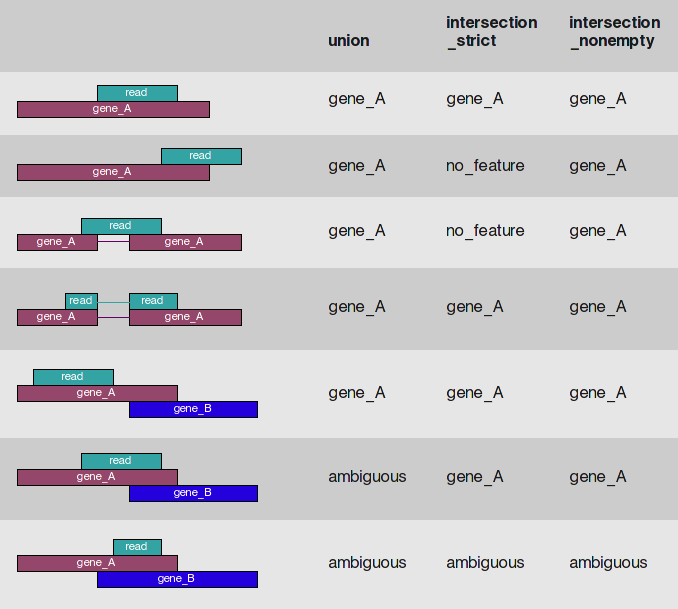
\includegraphics[width=10cm,height=7cm,keepaspectratio]{img/countmodes.png}
                \caption{HTSeq count modes - Source: HTSeq WebSite}
            \end{figure}
        \end{textblock*}
    }
\end{frame}

\begin{frame}
    \frametitle{Now HTSeq - transcription start sites}
    \begin{itemize}
        \item Compute a 'window' profile from an interval with respect to some features
    \end{itemize}
\end{frame}


\section{Investigations}

\begin{frame}
    \frametitle{Playing with HTSeq and different files}
    \begin{itemize}
        \item Realize that in practice you can't find real SAM files
        \item BAM files have at least 2GB size
        \item Samtools doesn't work very well when it comes to converting BAM to SAM
        \item Managed to get a QA plot
    \end{itemize}
\end{frame}

\begin{frame}
    \frametitle{Playing with HTSeq and different files}
    \begin{textblock*}{10cm}(1cm, 1cm)
        \begin{figure}
            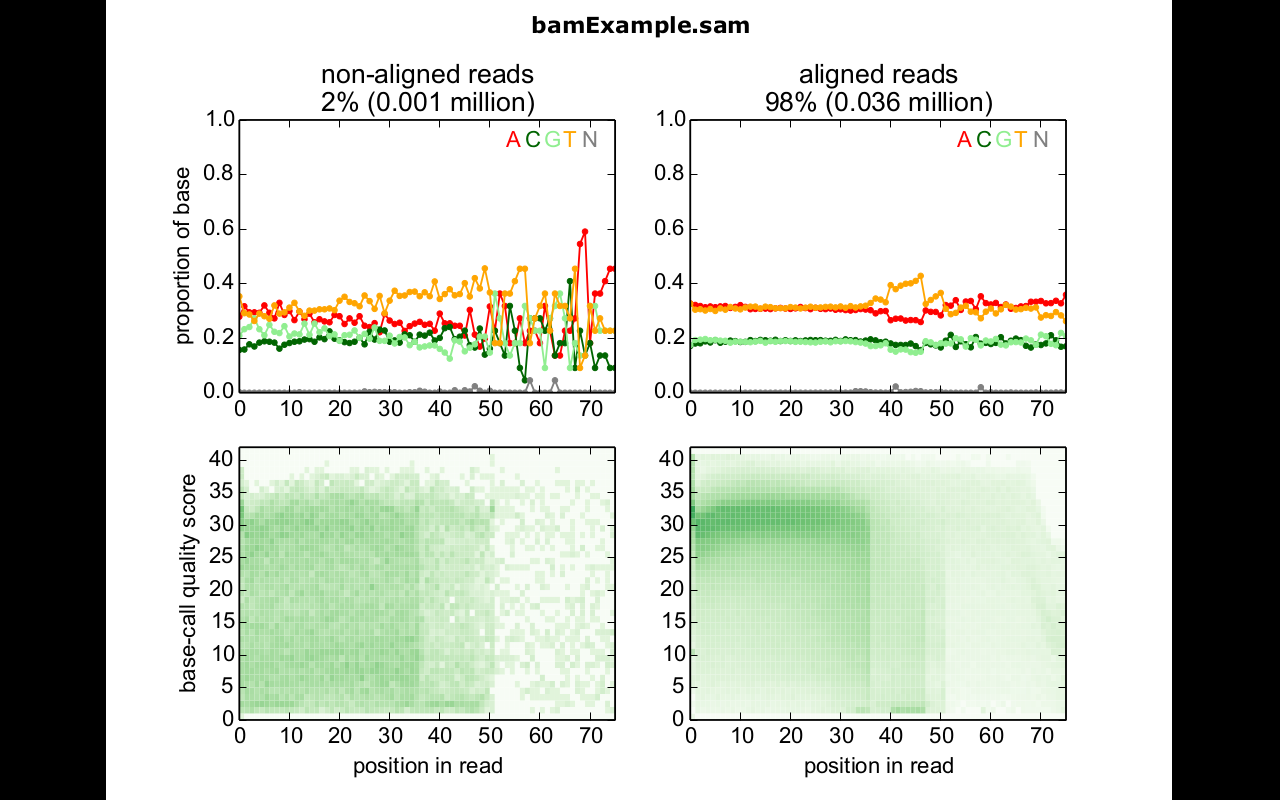
\includegraphics[width=10cm,height=7cm,keepaspectratio]{img/toyexample.png}
            \caption{Toy Example}
        \end{figure}
    \end{textblock*}
\end{frame}

\begin{frame}
    \frametitle{HTSeq}
    Live demonstration
\end{frame}

\begin{frame}
    \frametitle{Conclusions}
    \begin{itemize}
        \item HTSeq is a strong tool for manipulating High-Throughput data
        \pause
        \item Often, theory differs from practice
    \end{itemize}
\end{frame}

\begin{frame}
    \Huge{\centerline{Thank you!}}
\end{frame}

%\begin{frame}
%    Take some FASTQ files, perform quality asessement
%    Get some count of genes; mainly using htseq-count and qa
%    GFF - general feature format (former gene finding format) Not very well defined
%\end{frame}

%----------------------------------------------------------------------------------------

\end{document}
